% !TEX encoding = UTF-8 Unicode
\documentclass[a4paper]{article}

\usepackage[utf8]{inputenc}
\usepackage[T1]{fontenc}
\usepackage[slovene]{babel}
\usepackage{erk}
\usepackage{times}
\usepackage{graphicx}
\usepackage[top=22.5mm, bottom=22.5mm, left=22.5mm, right=22.5mm]{geometry}
\usepackage{array, booktabs}
\usepackage{amsmath}
\usepackage{url}

\graphicspath{{figures/}}
\def\footnotemark{}
\setlength{\emergencystretch}{2em}

\begin{document}
\sloppy

\title{Rehabilitacijski robot s prilagodljivo CMP pomočjo}

\author{Domen Brčar, Jakob Čehovin}

\affiliation{Fakulteta za elektrotehniko, Univerza v Ljubljani, Tržaška cesta 25, 1000 Ljubljana}

\email{E-mail: domen.brcar@student.uni-lj.si, jakob.cehovin@student.uni-lj.si}

\maketitle

\begin{abstract}{Povzetek}
Članek opisuje izvedbo rehabilitacijske naloge na robotu Franka Emika Panda,
kjer je gib opisan z dinamičnimi gibalnimi primitivami (DMP), mehka pomoč pa
z naučenimi kompenzacijskimi navori CMP. Cilj ni samo ponoviti demonstrirano
trajektorijo, temveč omogočiti nastavljivo pomoč glede na sposobnost uporabnika.
V končni programski verziji se posname začetna lega, iz demonstracij se
zgradi DMP referenca, iz meritev navorov se nauči CMP profil, izvedba pa
skalira dodani navor z enim parametrom sposobnosti. Uporabljene so
štiri trajektorije: osnovni premik in tri poti za zaporedje z žogico. Za vsako
pot žogice sta pripravljena ločena CMP signala za gib naprej in povratek po
isti poti. Sistem med prehodi ne preide v popolno podajnost, ampak stabilno
drži trenutno oziroma ciljno lego.
\end{abstract}

\section{Uvod}

Robotska rehabilitacija zgornje okončine temelji na ponovljivem izvajanju
nalog, merjenju odziva in varni fizični interakciji z uporabnikom. Klinični
pregledi poročajo, da lahko elektromehanski oziroma robotski sistemi po
možganski kapi izboljšajo aktivnosti vsakdanjega življenja, funkcijo roke in
mišično moč, vendar so učinki odvisni od izvedbe terapije, doziranja in
značilnosti uporabnika~\cite{mehrholz2018cochrane}. Klasična dela s področja
robot-aided neurorehabilitation zato poudarjajo ponovljivost, merljivost in
interaktivno vodenje kot glavne prednosti robotskih sistemov~\cite{krebs1998robot}.

Pri sodelovanju človeka in robota sama natančnost sledenja ni dovolj. Robot
mora nalogo izvajati dovolj stabilno, da ne ogroža uporabnika, hkrati pa ne
sme postati tog manipulator, ki bi uporabniku odvzel aktivno vlogo. To je
razlog, da je v projektu uporabljen koncept pomoči po potrebi: referenčna
trajektorija je vedno določena, dodatni navor pa je nastavljiv in omejen.
Takšen pristop se naravno navezuje na impedančno vodenje, kjer robot ni opisan
le kot sledilnik položaja, temveč kot mehanski sistem z izbrano togostjo,
dušenjem in vztrajnostjo~\cite{hogan1985impedance}.

Za zapis referenčnih gibov so uporabljene dinamične gibalne primitive (DMP).
DMP so stabilni nelinearni dinamični sistemi, ki ločijo osnovno privlačno
dinamiko od naučenega nelinearnega člena. Zato lahko iz ene demonstracije
zapišejo gladek gib, ga reproducirajo z enako končno točko in ga po potrebi
časovno skalirajo~\cite{schaal2006dmp,ijspeert2013dmp}. Novejši pregled
Saveriana idr. DMP umešča med standardna orodja učenja iz demonstracije,
interakcije z okoljem in robotike v kontaktu~\cite{saveriano2023dmp}.

\section{DMP zapis giba}

Diskretni DMP za en sklep je zapisan s kanonično fazno spremenljivko $x$ in
transformacijskim sistemom za položaj $y$. Faza pada od $1$ proti $0$:
\begin{equation}
    \tau \dot{x} = -a_x x ,
    \label{eq:canonical}
\end{equation}
kjer je $\tau$ trajanje giba. Transformacijski sistem je
\begin{equation}
    \tau \dot{z} = a_z \left(b_z (g-y) - z \right) + f(x),
    \qquad
    \tau \dot{y} = z .
    \label{eq:transform}
\end{equation}
Pri $b_z=a_z/4$ je osnovni del kritično dušen sistem, ki konvergira proti
cilju $g$. Naučeni člen $f(x)$ doda obliko demonstrirane trajektorije:
\begin{align}
    f(x) &=
    x\frac{\sum_{i=1}^{N} \psi_i(x) w_i}
         {\sum_{i=1}^{N} \psi_i(x)}, \nonumber\\
    \psi_i(x) &= \exp\left(-\frac{(x-c_i)^2}{2\sigma_i}\right).
    \label{eq:forcing}
\end{align}
Uteži $w_i$ se določijo z najmanjšimi kvadrati iz demonstracije
$q(t),\dot{q}(t),\ddot{q}(t)$. V implementaciji se to naredi ločeno za vseh
sedem sklepov robota Panda. Demonstracija se najprej prebere iz datoteke
\texttt{.npz}, nato se izgradi matrika baznih funkcij, rešitev linearnega
sistema pa določi DMP uteži. Isti postopek se uporablja za osnovni premik in
za tri trajektorije naloge z žogico.

Prednost DMP v tem projektu je praktična. Referenca ni neposredno surov
posnetek, ampak zglajen dinamični model. Robot zato dobi zvezen potek
$q_\mathrm{ref}(t)$ in $\dot{q}_\mathrm{ref}(t)$, kar zmanjša sunkovite ukaze
pri izvedbi. DMP hkrati ne zahteva popolnega modela robota ali uporabnika;
zadostuje demonstracija v sklepnem prostoru. To je primerno za laboratorijsko
rehabilitacijsko nalogo, kjer je cilj ponovljiva vaja, ne splošno načrtovanje
poljubnih gibov.

\section{CMP pomoč}

Klasični DMP opisuje kinematiko giba. Pri nalogah v kontaktu pa sama pot ne
pove, kakšni navori so potrebni za varno in dovolj natančno izvedbo. CMP
(compliant movement primitives) zato razširijo idejo primitiv: poleg
kinematične poti se nauči še dinamični oziroma navorni del naloge. Pregled
Deniše idr. CMP opisuje kot okvir, kjer se z DMP zapiše želena kinematika,
task-dependent dinamika pa se modelira z navorno primitivo~\cite{denisa2016cmp}.
Sorodna dela z gibanjem v kontaktu kažejo, da je vključevanje interakcijskih
signalov ključno, ko robot ne deluje v praznem prostoru~\cite{gams2014coupling}.

V izvedbi projekta se CMP uči eksperimentalno. Robot najprej izvede DMP
referenco v togem oziroma kontroliranem načinu, med izvedbo pa se shranijo
merjeni sklepi, hitrosti in navori. Izmerjeni navori $\tau_m(t)$ se nato
zapišejo z enakim DMP postopkom kot položaji. Rezultat je gladek profil
$\tau_\mathrm{CMP}(t)$, ki se pri kasnejši rehabilitacijski izvedbi doda kot
feedforward pomoč:
\begin{equation}
    \tau_d(t) = \tau_\mathrm{ramp}(t)\,
    k_\mathrm{CMP}\,\alpha\,\tau_\mathrm{CMP}(t).
    \label{eq:tauadd}
\end{equation}
Parameter
\begin{equation}
    \alpha=\frac{100-\mathrm{SPOSOBNOST}}{100}
    \label{eq:alpha}
\end{equation}
pretvori uporabniško nastavitev v delež pomoči. Pri vrednosti 0 je
$\alpha=1$, pri vrednosti 100 pa je
$\alpha=0$. Dodani navor se pred pošiljanjem robotu omeji:
\begin{equation}
    \tau_d(t) = \mathrm{clip}\left(\tau_d(t),
    -\tau_\mathrm{lim},\tau_\mathrm{lim}\right).
    \label{eq:clip}
\end{equation}
Rampa $\tau_\mathrm{ramp}(t)$ na začetku in koncu giba prepreči skokovito
vklapljanje pomoči. V trenutni nastavitvi je uporabljena meja
$\tau_\mathrm{lim}=4$ Nm, faktor CMP pa je odvisen od sposobnosti uporabnika.

Pomembna odločitev v verziji \texttt{sposobnost v4} je, da se za povratni gib
ne uporabi samo negiran ali časovno obrnjen CMP signal. Za vsako trajektorijo
žogice je shranjen ločen signal za smer naprej in smer nazaj. To je skladno s
prakso DMP, kjer povratni gib ni nujno dinamično enak obratni smeri; drugačen
kontakt, gravitacijski prispevek in začetna lega lahko zahtevajo drugačen
navorni profil.

\section{Programsko okolje}

Projekt je urejen v tri glavne mape. V mapi \texttt{src} sta glavni notebook
verzije v4 in podporni datoteki \texttt{dmp.py} ter \texttt{utils.py}.
Podmapa s trajektorijami vsebuje le podatke, ki jih uporablja končni program:
začetno točko, štiri posnete trajektorije in sedem CMP datotek. Fotografije so
v mapi \texttt{pictures}; originali HEIC so pretvorjeni v JPG, kontaktna slika
pa je vključena v poročilo.

Notebook je razdeljen na logične sklope:
\begin{enumerate}
    \item inicializacija robota Panda in prijemala,
    \item nastavitev poti, trajektorij, CMP datotek in parametra sposobnosti,
    \item funkcije za snemanje, učenje DMP, učenje CMP in izvedbo,
    \item snemanje začetne lege ter demonstracij,
    \item nalaganje referenc, učenje oziroma nalaganje CMP signalov,
    \item izvedba osnovnega premika in cikla žogica 1--2--3,
    \item shranjevanje rezultatov in izris.
\end{enumerate}

Pri izvedbi se robot pred vsakim gibom premakne v začetno točko reference,
jo kratek čas stabilno drži, nato izvede referenco z dodatnim CMP navorom.
Po koncu giba robot ne preklopi v popolno podajnost, temveč drži zadnjo ciljno
lego. Ta del je bil v projektu ključen, ker se pri zaporedju več trajektorij
napake in prehodi sicer hitro poznajo kot padec roke ali neželen preskok med
stanji.

\section{Podatki in rezultati}

Eksperimentalna postavitev je prikazana na sliki~\ref{fig:fotografije}. Slike
so bile posnete v formatu HEIC in pretvorjene v JPG, ker je to robustnejši
format za vključitev v \LaTeX. Tehnična vsebina poročila pa temelji na
dejanskih datotekah \texttt{.npz}, ne na ročnem prepisovanju meritev.

\begin{figure}[!htb]
    \begin{center}
        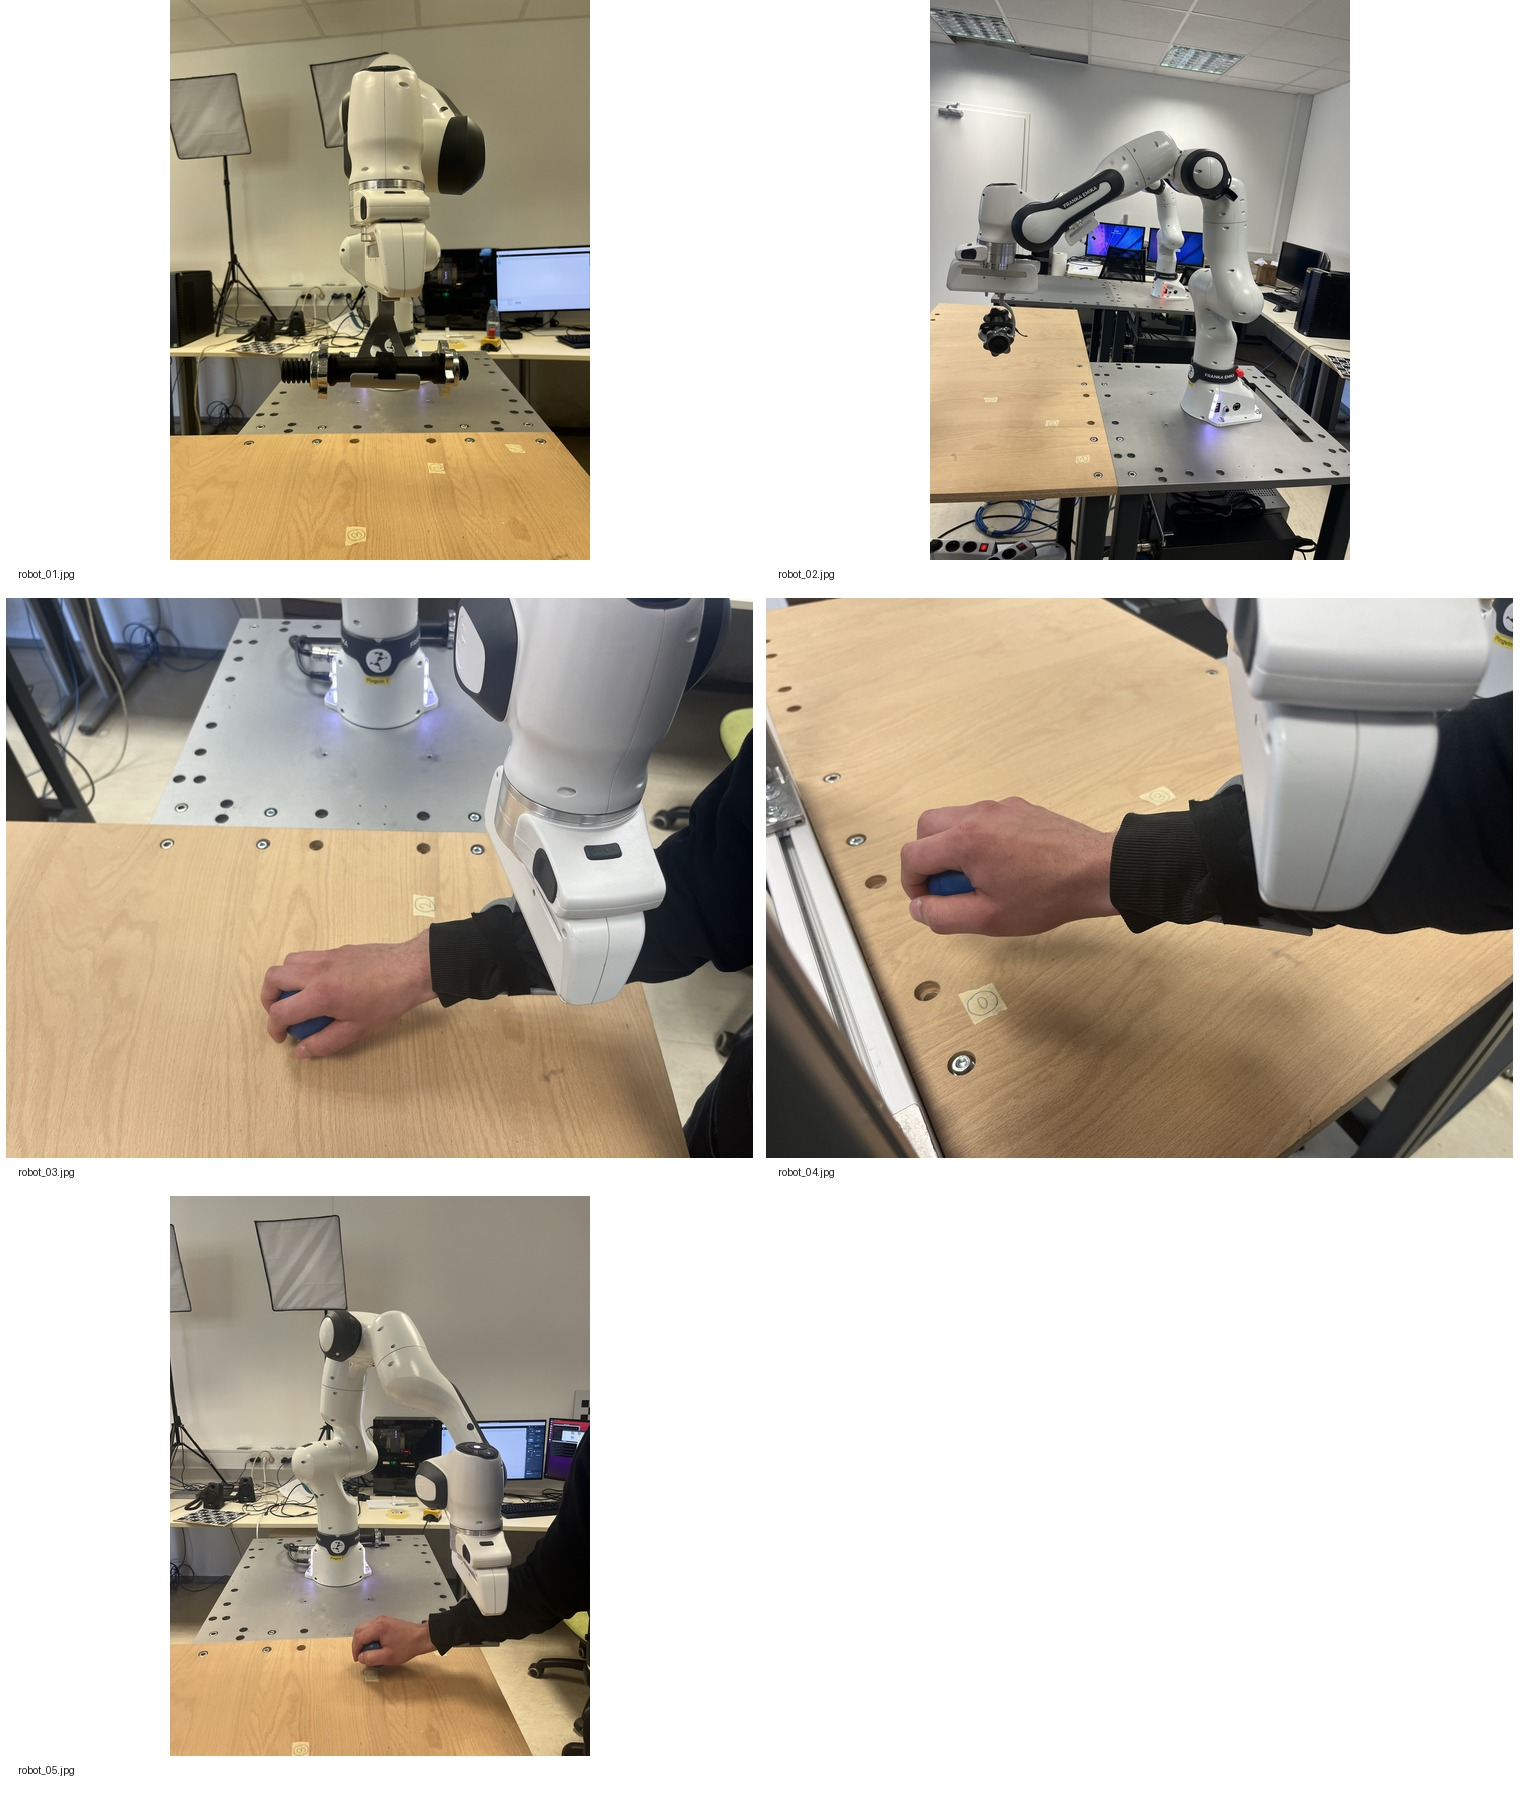
\includegraphics[width=\columnwidth]{robot_fotografije_kontakt.jpg}
        \caption{Eksperimentalna postavitev rehabilitacijske naloge z robotom Panda.}
        \label{fig:fotografije}
    \end{center}
\end{figure}

\begin{table}[htbp]
    \centering
    \caption{Povzetek uporabljenih trajektorij}
    \label{tab:trajektorije}
    \begin{tabular}{lccc}
        \toprule
        Trajektorija & Vzorci & Trajanje [s] & Sklepi \\
        \midrule
        Premik & 599 & 5.98 & 7 \\
        Žogica 1 & 804 & 8.03 & 7 \\
        Žogica 2 & 610 & 6.09 & 7 \\
        Žogica 3 & 585 & 5.84 & 7 \\
        \bottomrule
    \end{tabular}
\end{table}

Tabela~\ref{tab:trajektorije} kaže, da so vse demonstracije počasne in
primerne za rehabilitacijsko izvedbo. Najdaljša je prva trajektorija žogice,
ki traja 8.03 s, osnovni premik pa traja 5.98 s. Število vzorcev je skladno s
frekvenco snemanja 100 Hz. Povzetek je prikazan tudi na sliki
\ref{fig:povzetek}.

\begin{figure}[!htb]
    \begin{center}
        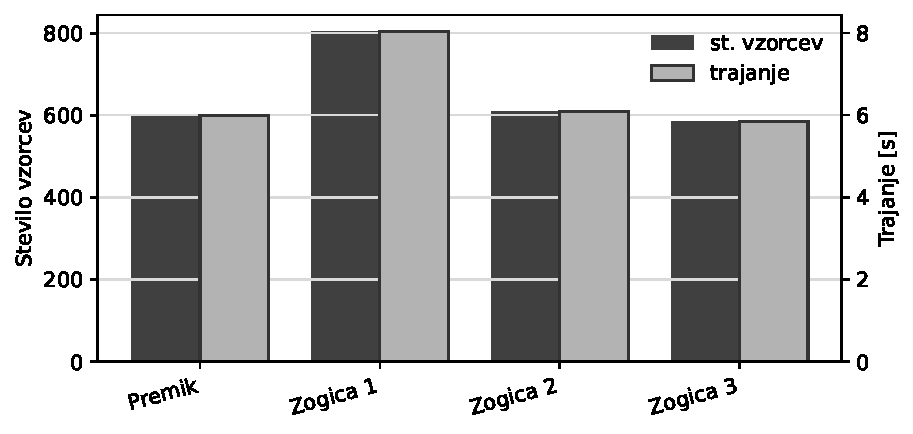
\includegraphics[width=\columnwidth]{povzetek_trajektorij.pdf}
        \caption{Število vzorcev in trajanje posnetih trajektorij.}
        \label{fig:povzetek}
    \end{center}
\end{figure}

Sklepni poteki na sliki~\ref{fig:sklepi} potrjujejo, da so trajektorije dovolj
gladke za DMP zapis. Največ sprememb je v sklepih, ki prispevajo k premiku
končnega efektorja po delovni površini; ostali sklepi predvsem držijo
konfiguracijo roke. Pri rehabilitacijski izvedbi je to zaželeno, ker se naloga
osredotoča na vodeno premikanje končnega efektorja, ne na iskanje nove
kinematične konfiguracije.

\begin{figure}[!htb]
    \begin{center}
        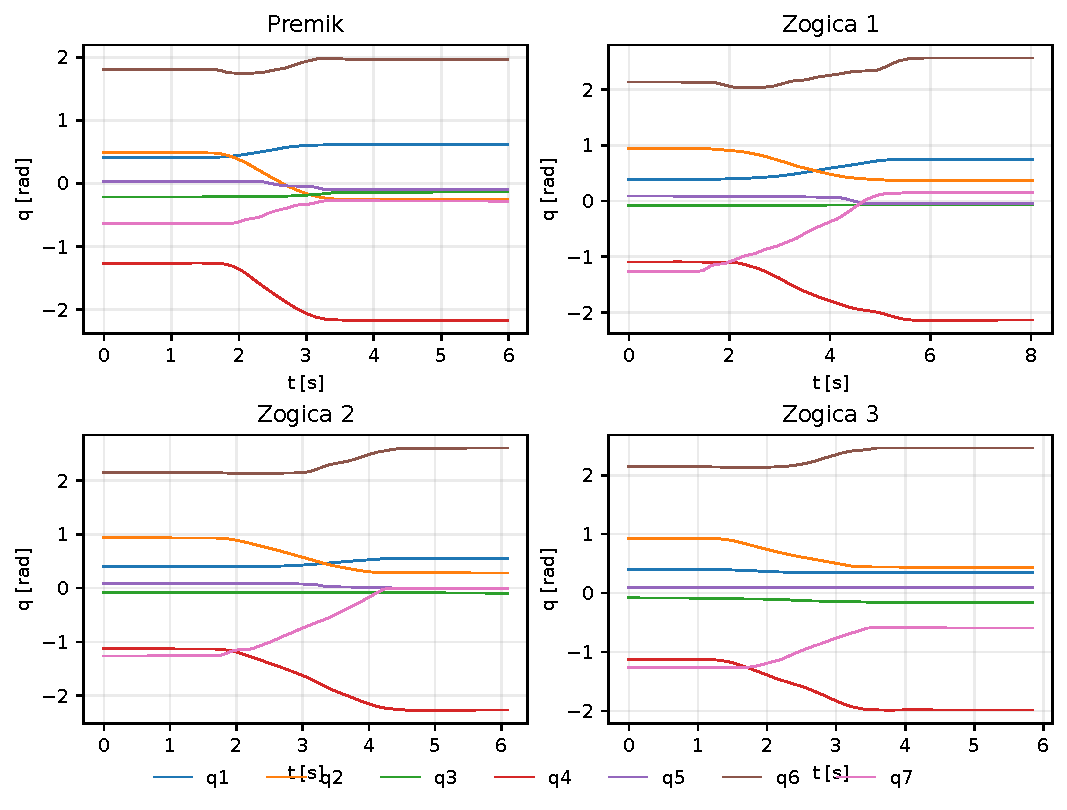
\includegraphics[width=\columnwidth]{trajektorije_sklepi.pdf}
        \caption{Sklepni poteki osnovnega premika in treh trajektorij žogice.}
        \label{fig:sklepi}
    \end{center}
\end{figure}

Slika~\ref{fig:cmp} prikazuje normo CMP navorov. Norme niso neposredno ukazani
navori pri vsaki izvedbi, ampak naučeni profili pred skaliranjem s
\texttt{SPOSOBNOST}. Če je sposobnost uporabnika večja, se celoten profil
zmanjša; če je sposobnost manjša, se profil ohrani bližje naučeni vrednosti,
vendar ga še vedno omeji meja \eqref{eq:clip}. Ločeni profili naprej in nazaj
so uporabni predvsem pri zaporedju žogica 1--2--3, ker robot po vsaki poti
stabilno pride nazaj v izhodišče za naslednji gib.

\begin{figure}[!htb]
    \begin{center}
        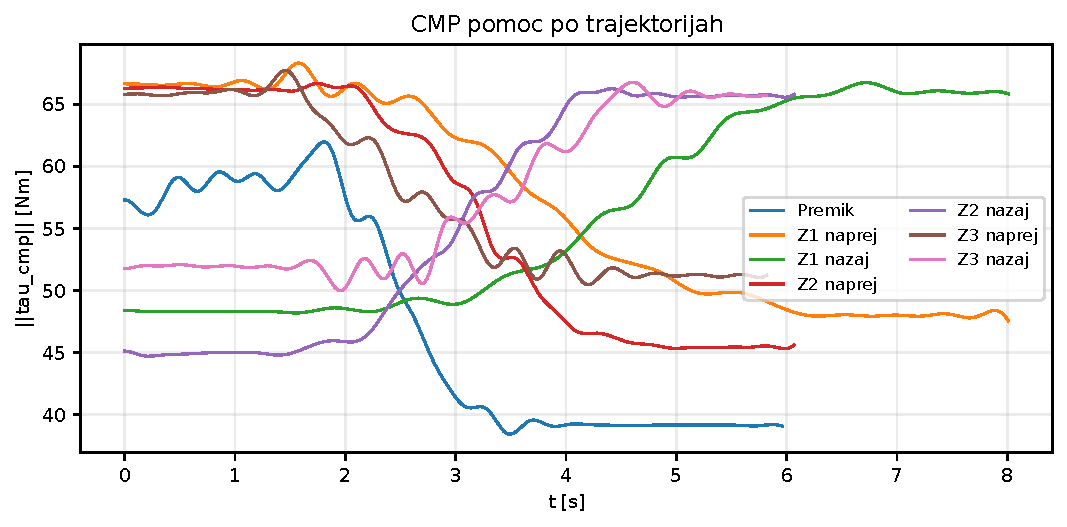
\includegraphics[width=\columnwidth]{cmp_norme.pdf}
        \caption{Norma naučenih CMP navorov za osnovni premik in trajektorije žogice.}
        \label{fig:cmp}
    \end{center}
\end{figure}

\section{Razprava}

Glavna tehnična vrednost projekta je ločitev med kinematično referenco in
dinamično pomočjo. DMP poskrbi za ponovljivo, gladko pot; CMP pa doda
navorni prispevek, ki ga je mogoče skalirati. Takšna arhitektura je boljša od
ene same toge reference, ker omogoča več režimov vadbe brez ponovnega snemanja
trajektorij. Isti nabor podatkov je uporaben za popolnejšo pomoč začetniku in
za manjšo pomoč uporabniku, ki že zmore večji del giba sam.

Druga pomembna odločitev je stabilizacija prehodov. Pri zaporednih nalogah
robot ne sme med koncem ene poti in začetkom naslednje nenadzorovano popustiti.
Zato notebook pred začetkom, med prehodi in po koncu trajektorije uporablja
držanje ciljne lege. To ni kozmetičen popravek, temveč varnostni pogoj za
laboratorijsko delo z realnim robotom.

Omejitev trenutne verzije je, da parameter sposobnosti določi
operater in je med poskusom konstanten. Bolj napredna rešitev bi sproti
ocenjevala uporabnikov prispevek iz napake sledenja, merjenih navorov ali
interakcijske sile. Takrat bi lahko $\alpha$ v enačbi~\eqref{eq:alpha}
postala časovno spremenljiva vrednost. Dodatna nadgradnja bi bila filtriranje
CMP signalov glede na utrujenost uporabnika, saj enak navorni profil na
začetku in koncu terapije ni nujno enako primeren.

Trenutni rezultati so zato predvsem validacija programske strukture in
podatkovnega toka. Projekt ima pripravljeno osnovo za eksperimentalno
primerjavo različnih vrednosti sposobnosti, za merjenje napake
sledenja in za oceno, pri kateri nastavitvi uporabnik še aktivno sodeluje.

\section{Zaključek}

Končna verzija projekta združuje DMP reference, CMP navorno pomoč in stabilno
izvedbo zaporedja trajektorij. Podatki so urejeni v ločeno mapo, fotografije
so pretvorjene v poročilu uporaben format, članek pa povzema metodo brez
odvisnosti od starih razvojnih notebookov. Najpomembnejša funkcionalnost je
parameter \texttt{SPOSOBNOST}, ki iz ene naučene trajektorije in enega CMP
profila omogoči več stopenj robotske pomoči. S tem je projekt pripravljen za
naslednji korak: sistematično testiranje uporabnikovega sodelovanja in
adaptivno prilagajanje pomoči med vadbo.

\small
\bibliographystyle{ieeetr}
\bibliography{references}

\end{document}
